% Это основная команда, с которой начинается любой \LaTeX-файл. Она отвечает за тип документа, с которым связаны основные правил оформления текста.
\documentclass[a4paper,12pt]{extarticle}

\usepackage{geometry}
\usepackage[T1]{fontenc}
\usepackage[utf8]{inputenc}
\usepackage[english,russian]{babel}
\usepackage{amsmath}
\usepackage{amsthm}
\usepackage{amssymb}
\usepackage{fancyhdr}
\usepackage{setspace}
\usepackage{graphicx}
\usepackage{colortbl}
\usepackage{tikz}
\usepackage{pgf}
\usepackage{subcaption}
\usepackage{indentfirst}
\usepackage[
backend=biber,
style=numeric,
maxbibnames=99
]{biblatex}
\addbibresource{Bibliography/sources.bib}
\usepackage{indentfirst}
\usepackage{mathtools}
\usepackage{booktabs}
\usepackage[flushleft]{threeparttable}
\usepackage{tablefootnote}
\usepackage{microtype}
\pretolerance=1000 % Adjust the threshold for line breaking


\usepackage{chngcntr} % нумерация графиков и таблиц по секциям
\counterwithin{table}{section}
\counterwithin{figure}{section}

\graphicspath{{graphics/}}%путь к рисункам

\makeatletter
% \renewcommand{\@biblabel}[1]{#1.} % Заменяем библиографию с квадратных скобок на точку:
\makeatother

\geometry{left=2.5cm}% левое поле
\geometry{right=1.0cm}% правое поле
\geometry{top=2.0cm}% верхнее поле
\geometry{bottom=2.0cm}% нижнее поле

\setlength{\parindent}{1.25cm}
\renewcommand{\baselinestretch}{1.5} % междустрочный интервал
\setlength{\footnotesep}{0.9\baselineskip}


% Пакеты для отображения картинок
\usepackage{graphicx}
\usepackage{float}
\usepackage{wrapfig}

\usepackage[breaklinks, unicode=true, colorlinks=true, linkcolor=blue, urlcolor=blue,citecolor=blue]{hyperref}
\usepackage{xurl}

\usepackage{setspace}
% \renewcommand{\theenumi}{\arabic{enumi}}% Меняем везде перечисления на цифра.цифра
% \renewcommand{\labelenumi}{\arabic{enumi}}% Меняем везде перечисления на цифра.цифра
% \renewcommand{\theenumii}{.\arabic{enumii}}% Меняем везде перечисления на цифра.цифра
% \renewcommand{\labelenumii}{\arabic{enumi}.\arabic{enumii}.}% Меняем везде перечисления на цифра.цифра
% \renewcommand{\theenumiii}{.\arabic{enumiii}}% Меняем везде перечисления на цифра.цифра
% \renewcommand{\labelenumiii}{\arabic{enumi}.\arabic{enumii}.\arabic{enumiii}.}% Меняем везде перечисления на цифра.цифра

\setcounter{biburllcpenalty}{7000}
\setcounter{biburlucpenalty}{8000}

% \addbibresource{Bibliography/sources.bib}

\setlength{\parskip}{6pt}
\setlength{\parindent}{10pt}

\usepackage{pdfpages}

\usepackage{listings}

\lstdefinelanguage{Rust}{
  sensitive=true,
  morekeywords=[1]{
    break, continue, else, for, if, loop, match, return, while, struct
  },
  morekeywords=[2]{
    crate, fn, async, mod, pub, use, self, Self, struct, enum, const, static, let, mut, ref, type, impl, trait, where, as, dyn, move,
  },
  morekeywords=[3]{
    bool, char, i8, i16, i32, i64, isize, u8, u16, u32, u64, usize, f32, f64, str, String,
  },
  morekeywords=[4]{
    Ok, Err, Some, None,
  },
  morekeywords=[5]{
    await,
  },
  keywordstyle=[5]{\color{purple}},
  morecomment=[s]{/*}{*/},
  morecomment=[l]//,
  morestring=[b]",
  morestring=[b]r",
  morestring=[b]'',
}

\lstset{
  language=Rust,
  basicstyle=\ttfamily,
  keywordstyle=\color{blue},
  stringstyle=\color{red},
  commentstyle=\color{green},
  showstringspaces=false,
  breaklines=true,
  frame=none,
}


\lstnewenvironment{rustcode}[1][]{
  \lstset{
    language=Rust,
    basicstyle=\ttfamily,
    keywordstyle=\color{blue},
    stringstyle=\color{red},
    commentstyle=\color{gray},
    showstringspaces=false,
    breaklines=true,
    % frame=single,
    #1
  }
}{}


\lstnewenvironment{cppcode}[1][]{
  \lstset{
    language=C++,
    basicstyle=\ttfamily,
    keywordstyle=\color{blue},
    stringstyle=\color{red},
    commentstyle=\color{gray},
    showstringspaces=false,
    breaklines=true,
    % frame=single,
    #1
  }
}{}


\newcommand{\thisdate}{17.05.2023}


% С этого момента начинается текст документа
\begin{document}

% Эта команда создает титульную страницу

% \makeTitlePage

\begin{titlepage}
\newpage

{\setstretch{1.0}
\begin{center}
ПРАВИТЕЛЬСТВО РОССИЙСКОЙ ФЕДЕРАЦИИ\\
ФГАОУ ВО НАЦИОНАЛЬНЫЙ ИССЛЕДОВАТЕЛЬСКИЙ УНИВЕРСИТЕТ\\
«ВЫСШАЯ ШКОЛА ЭКОНОМИКИ»
\\
\bigskip
Факультет компьютерных наук\\
Образовательная программа «Прикладная математика и информатика»
\end{center}
}

\vspace{2em}
\vspace{5em}

\begin{center}
%Выберите какой у вас проект
{\bf Отчет о программном проекте на тему:}\\
%{\bf Отчет о программном проекте на тему:}\\
{\bf Реализация поддержки асинхронного программирования для фреймворка DSLab}
\end{center}

\vspace{2em}

{\bf Выполнил: \vspace{2mm}}


{\setstretch{1.0}
\begin{tabular}{l@{\hskip 1.5cm}c@{\hskip 1.5cm}c}
студент группы БПМИ206 & & \thisdate \\
Макогон Артём Аркадьевич & \rule{3.5cm}{0.15mm}  &  \rule{3.5cm}{0.15mm} \vspace{-2mm} \\
    & \tiny{(подпись)}  & \tiny{(дата)} \\
\end{tabular}}

\vspace{1em}
{\bf Принял руководитель проекта: \vspace{2mm}}

{\setstretch{1.0}
\begin{tabular}{l@{\hskip 1.5cm}l}
Сухорослов Олег Викторович \\
Кандидат технических наук, доцент \\
Факультета компьютерных наук НИУ ВШЭ \vspace{10mm}\\
  & \hspace{1cm}\thisdate\\
\rule{4cm}{0.15mm}  &  \rule{4cm}{0.15mm} \vspace{-2mm}\\
{\hskip 1.5cm}\tiny{(подпись)} & {\hskip 1.5cm}\tiny{(дата)} \\
\end{tabular}}

\vspace{\fill}

\begin{center}
Москва 2023
\end{center}

\end{titlepage}


% \newpage

\setcounter{page}{2}
{
\hypersetup{linkcolor=black}
% Здесь будет автоматически генерироваться содержание документа
\tableofcontents
}

\newpage
%!TEX root=../main.tex

\section*{Аннотация}

Современные информационные и вычислительные системы все чаще становятся распределенными из-за увеличения объема вычислений и данных, а также требований к производительности и масштабируемости. Исследования по алгоритмическому обеспечению распределенных систем проводятся для разработки эффективных алгоритмов управления ресурсами, планирования задач, балансировки нагрузки и других задач. Аналитические и имитационные модели используются для упрощения и ускорения экспериментов, изучения поведения таких систем в разных ситуациях.
\texttt{DSLab} -- программный фреймворк для имитационного моделирования и тестирования распределенных систем, предоставляющий множество возможностей как для написания новых алгоритмов, так и использования готовых модулей. В основе любой симуляции \texttt{DSLab} лежит дискретно-событийный подход описания моделей и приложений, где события обрабатываются в пользовательских функциях (\texttt{callback}-ах). В рамках проекта добавлена возможность управлять событиями асинхронно, а также комбинировать эти подходы. Благодаря новому функционалу можно писать более выразительный и понятный код, что ускоряет процесс разработки алгоритмов и делает фреймворк более привлекательным для исследователей. 

\section*{Ключевые слова}

Распределенные системы, симуляция, асинхронность, DSLab


\newpage 

\section{Основные термины и определения}

\begin{enumerate}
    \item Распределенная система -- система, выполняющая определенную задачу по обработке данных и компьютерных вычислений и использующая для этого несколько независимых машин (узлов), каждый из которых обладает своими ресурсами, памятью и запущенными процессами.
    \item Симуляция -- это процесс исполнения имитационной модели реальной системы или процесса, которая может быть использована для изучения и предсказания поведения системы в различных условиях.
    \item DSLab -- программный фреймворк для имитационного моделирования и тестирования распределенных систем.
    \item Асинхронное программирование -- это парадигма программирования, основанная на неблокирующем ожидании, которое позволяет программам переключаться на выполнение других задач в ожидании длительных операций.
    \item Callback -- это функция или код, который передается в качестве аргумента другой функции или метода, для выполнения в более поздний момент в ответ на событие или операцию.
    \item Логирование -- хронологическая запись операций, выполненных в системе. Логирование позволяет сохранять информацию о состоянии системы, которую можно использовать для ее исследования и отладки.
\end{enumerate}

\newpage

\section{Введение}

\subsection{Описание предметной области}

Практически все современные информационные и вычислительные системы являются распределенными. Связано это с растущими объемами вычислений и обрабатываемых данных, требованиями к производительности, надежности и масштабируемости. Алгоритмическое обеспечение распределенных систем (например, алгоритмы управления ресурсами, планирования задач, балансировки нагрузки, членства в группе, консенсуса) является предметом активных исследований. В силу масштабов современных систем, сложности их реализации и недетерминированного характера, исследование алгоритмов и тестирование их реализаций в реальных системах существенно затруднено. Поэтому часто подобные исследования проводятся на аналитических и имитационных моделях, описывающих существенные для решаемой задачи аспекты поведения системы и проводимых вычислений. Использование моделей позволяет значительно удешевить эксперименты, сократить время их проведения и обеспечить воспроизводимость их результатов.

\texttt{DSLab}\cite{dslab-repo} предлагает широкий набор инструментов для тестирования различных алгоритмов. Более подробно про проект можно прочитать в его описании \cite{dslab-description}, его требования \cite{dslab-requirements} и сравнение с аналогами \cite{dslab-analog-cmp}.

\subsection{Архитектура проекта DSLab}

В силу широты охвата областей применения фреймворка он организован в виде набора слабо связанных программных модулей, использование которых будет осуществляться через их API. Это даст возможность пользователям фреймворка (исследователям, разработчикам, преподавателям) гибким образом собирать из модулей решения под свои цели, например симуляторы для конкретных типов систем или постановок задач.

Входящие в состав фреймворка модули можно условно разделить на три типа:
\begin{enumerate}
    \item 
    Базовые, функциональность которых используется остальными модулями (например, 
    
    реализация дискретно-событийного моделирования);
    \item
    Универсальные, функциональность которых может быть использована в различных предметных областях (например, модели сети);
    \item
    Специализированные, которые заточены под определенную предметную область (например, библиотеки для моделирования облачных инфраструктур, исследования алгоритмов планирования заданий на кластерах или тестирования решений учебных заданий).
\end{enumerate}

Архитектуру DSLab можно схематично представить в виде трех слоев (Рис. \ref{dslab_arc}), включающих модули соответствующего типа. На рисунке также указаны текущие модули и зависимости между ними. Зависимости от \texttt{dslab-core} (от него зависят все имеющиеся универсальные и специализированные модули) не указаны, чтобы не загромождать рисунок. Таким образом, модули могут зависеть от модулей с нижних слоев, но не наоборот.

\begin{figure}[H]
    \centering
    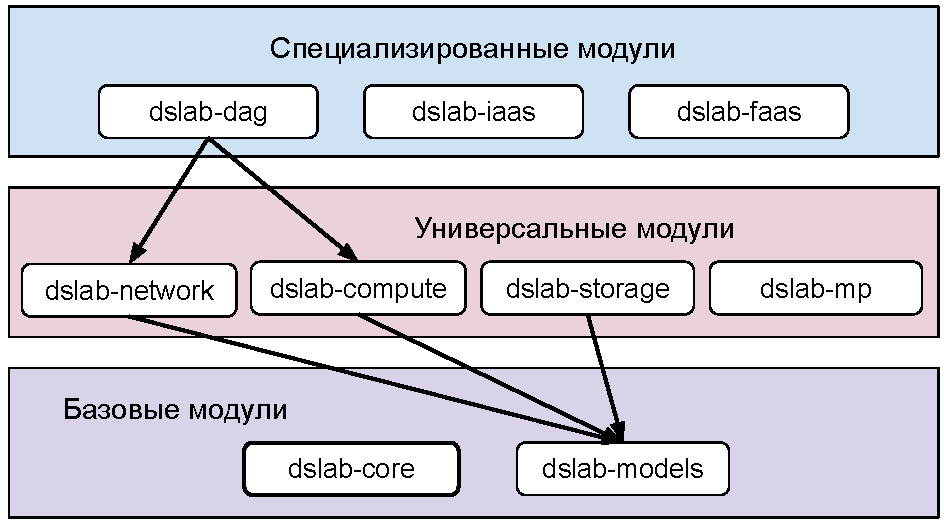
\includegraphics[width=0.7\linewidth]{images/dslab_arc}
    \caption{Архитектура DSLab}
    \label{dslab_arc}
\end{figure}

Описание архитектуры основано на документации проекта \cite{dslab-architecture}.  Реализации модулей представлены в основном репозитории \cite{dslab-repo}.

Таким образом пользователь при разработке собственной симуляции может либо использовать уже готовые разработанные компоненты, либо реализовывать свои и произвольно их связывать. 

Основным процессом в симуляции является создание событий и исполнения процессов реагирования на них. Разные компоненты генерируют события друг для друга и с помощью низкоуровневого модуля \texttt{dslab-core} обмениваются ими. Чтобы как-то реагировать на событие, каждый компонент реализует единственный обобщенный метод, в который \texttt{dslab-core} передает нужное событие. При обработке события компоненты генерируют новые и таким образом цикл симуляции замыкается. 

Получается, что сейчас реагировать на пришедшие события можно только в одном месте -- в той самой функции-\texttt{callback}, которую позовет \texttt{dslab-core}. В случае, когда событий немного, это лаконично выглядит, этим удобно пользоваться. Но в более сложных алгоритмах с большим количеством различных событий, и, что важнее, цепочками событий, на которые нужно последовательно реагировать, подобная модель становится не самой удобной. С такой единой точкой входа многие последовательные логичные действия оказываются фрагментированы (разбросаны по разным участкам кода, подробнее можно смотреть разбор примеров из главы \ref{async-testing}). 

Хотелось бы иметь альтернативную возможность писать на языке программирования более понятный с первого взгляда алгоритм. Как раз такой возможностью является написание асинхронного кода.


\subsection{Преимущества асинхронного подхода}

Для описания моделей, тестов и алгоритмов в фреймворке используется язык \texttt{Rust}, который на уровне языка поддерживает возможность писать асинхронный код. Главные преимущества асинхронной парадигмы программирования~--~удобство при написании сложных многоступенчатых алгоритмов и повышение читаемости кода. Процесс принятия решения о сохранении файла в распределенном хранилище в такой парадигме мог бы выглядеть таким образом (псевдокод):

\begin{figure}[H]
    \small
\begin{rustcode}
    async fn add_file_to_storage(some_file) {
        send_file_to_all_replicas(some_file);
        result = wait_for_confirmation_from_all().await;
        if result.has_quorum {
            send_commit_to_replicas(result.nodes);
            wait_for_commit_confirmation_from(result.nodes).await;
            send_ok_message_to_user();
        } else {
            send_reject_message_to_user();
        }
    }
\end{rustcode}
\caption{Псевдокод асинхронного взаимодействия нод в симуляции}
\label{pseudocode}
\end{figure}

Посмотрев на функцию можно понять, что она делает, потому что логика последовательна и удобно разбита на подфункции. Используя асинхронность, у нас есть возможность написать такой алгоритм на верхнем уровне. 

\subsection{Возможные недостатки асинхронного подхода}

Программировать в парадигме асинхронного взаимодействия требует соответствующей подготовки пользователя. Не смотря на то, что в любой момент времени исполняется только одна функция (подробнее о реализации см. в главе \ref{inner}), и проблем многопоточного программирования вида \texttt{data-race} не возникает, нужно постоянно держать в голове, что <<параллельно>> могут быть запущены другие процессы, которые могли поменять общую память в то время, когда функция была неактивна. 

\subsection{Постановка задачи}\label{main-purpose}
Целью является реализация поддержки асинхронного программирования для фреймворка \texttt{DSLab}. Для этого необходимо:
\begin{itemize}
    \item Реализовать асинхронное расширение для существующего ядра dslab-core.
    \item Добавить примеры использования нового функционала высокоуровневыми компонентами.
    \item Написать подробную документацию нового API и покрыть реализацию тестами.
\end{itemize}

\subsection{Полученные результаты}

После проделанной работы удалось добавить возможность управлять событиями в симуляции асинхронно. Были написаны схожие примеры с уже существующими, проведены замеры производительности и сравнение семантики получившегося кода(глава \ref{async-testing}). Код расширенного асинхронного ядра доступен в репозитории\cite{async-dslab-core}.


\section{Существующие работы и решения}

Подобный подход уже был реализован в других симуляторах, например в SimGrid\cite{simgrid-article}. Главное отличие подхода \texttt{DSLab} от \texttt{SimGrid} -- наличие дискретно-событийного моделирования. В \texttt{SimGrid} компоненты (акторы) общаются между собой асинхронно через \texttt{MailBox}-ы (аналог канала из языка Go). Код получается довольно объемный и непростой, но поскольку это самый близкий аналог, поддерживающий асинхронное программирование, его стоит разобрать. Ниже приведена (очень сокращенная) реализация самого простой примера процесса \texttt{ping-pong} в фреймворке \texttt{SimGrid}. Полный код примера можно посмотреть в репозитории\cite{simgrid-example}.
\begin{figure}[H]
    \centering
    \small
\begin{cppcode}
void Process(int id, Mailbox* in, vector<Mailbox*> peers, int iters) {
    // wait for Start message
    auto* msg = in->get<Message>();
    bool stopped = false;
    bool wait_reply = false;
    while (!stopped) {
        if (pings_to_send > 0 && !wait_reply) {
            MailBox* peer_mailbox = /* choose peer */;
            peer_mailbox->put_init(new Message(/*create message*/));
            wait_reply = true;
            pings_to_send -= 1;
        }
        msg = in->get<Message>();
        if (msg->type == MessageType::PING) {
            /* handle PING and send PONG back */
        } else if (msg->type == MessageType::PONG) {
            /* handle PONG and report Complete if applicable */
        } else if (msg->type == MessageType::STOP) {
            stopped = true;
        }
    }
}
\end{cppcode}
\caption{Код процесса \texttt{ping-pong} в фреймворке \texttt{SimGrid}}
\label{simgridcode}
\end{figure}

Из преимуществ сразу можно отметить, что процесс хранит свое состояние (количество оставшихся \texttt{ping}-ов, которые нужно сделать) на стеке функции и удобно его использует. Исполнение прерывается в методе \texttt{MailBox::get()} до момента получения сообщения. Подобный подход к асинхронности будет внедрен в \texttt{DSLab}.

Дальше можно выделить ряд недостатков, которых хотелось бы избежать. У этого процесса все еще единая точка входа (\texttt{MailBox* in}), и нужно обрабатывать все возможные варианты приходящего события. В этом плане нет большого различия с моделью \texttt{callback}-ов. Даже в более сложном примере \texttt{SimGrid-master-workers}\cite{simgrid-master-workers} все равно есть единая точка входа обработки событий, которые распределяются по хэндлерам на основе строки-префикса названия события.   
Также во всей симуляции некоторое количество кода уходит на ручное управление памятью (выделение c помощью \texttt{new} и освобождение с помощью \texttt{delete}). Такой подход повышает вероятность ошибки, и, как следствие, утечки памяти из симулятора. Это скорее является особенностью языка \texttt{C++}, а поскольку \texttt{DSLab} написан на \texttt{Rust}, подобной проблемы не предвидится.  


Альтернативной реализацией асинхронности в симуляции является использование корутин языка \texttt{Kotlin} в проекте \texttt{OpenDC}~\cite{opendc-repo}\cite{opendc-article}. К сожалению, проект не содержит достаточно разнообразных примеров использования симуляции в асинхронном контексте, но простой пример запуска симуляции~\cite{opendc-example} похож на ожидаемый опыт использования асинхронности в \texttt{DSLab}.


Опыт других проектов не очень хорошо подходит как опора для разработки нового решения из-за специфики языка \texttt{Rust} и внутренней архитектуры симулятора.

\section{Описание функциональных и нефункциональных требований к проекту}\label{requirements}

\subsection{Функциональные}
\begin{itemize}
    \item Код расширенного ядра должен иметь полную обратную совместимость со стандартным ядром, т.е. поддерживать возможность добавлять зависимости от уже реализованных модулей и программировать в модели \texttt{callback}-ов.
    \item Поддержка асинхронности должна предоставлять следующие возможности:
    \begin{itemize}
        \item запустить асинхронную задачу;
        \item остановить задачу на определенный промежуток времени внутри симуляции;
        \item асинхронно дождаться произвольного события от другого компонента;
        \item произвольно комбинировать ожидания используя методы из пакета \texttt{futures}\cite{rust-futures}.
    \end{itemize}
    \item Реализация должна содержать логирование происходящего в асинхронном контексте, а так же обработку ошибок, которая бы помогала пользователю искать ошибки в коде. 
\end{itemize}

\subsection{Нефункциональные}
\begin{itemize}
    \item Код проекта должен быть написан на языке Rust и опубликован как расширение модуля \texttt{dslab-core} в репозитории проекта \texttt{DSLab}\cite{dslab-repo}.
    \item Работа нового ядра должна быть продемонстрирована в использовании на разработанных примерах симуляций, в которых используется стандартная \texttt{callback-based} модель. Должны быть описаны преимущества и недостатки нового подхода.
    \item Расширение для ядра должно быть реализовано эффективно: не должны возникать дополнительные накладные расходы (асимптотически) по сравнению со стандартным ядром.
    \item Код должен быть написан в соответствии со стайлгайдом проекта \texttt{DSLab}
\end{itemize}




\section{Дизайн и структура ядра DSLab (dslab-core)} \label{dslab-core-design}

\subsection{Событие} \label{Event}
Основа дискретно-событийного моделирования -- события. В фреймворке DSLab они представлены структурой \underline{\texttt{Event}} со следующими полями: 
\begin{itemize}
    \item \texttt{id: EventId} -- уникальный идентификатор события во всей симуляции
    \item \texttt{time: f64} -- время наступления события 
    \item \texttt{src: Id} -- идентификатор компонента симуляции, создавшего это событие 
    \item \texttt{dest: Id} -- идентификатор компонента симуляции, которому это событие предназначается
    \item \label{Event:payload} \texttt{data: Box<dyn EventData>} -- произвольная <<полезная нагрузка>> события, которая может иметь любой тип и определяется пользователем. 
\end{itemize}

\subsection{Обработчик событий} \label{EventHandler}

Обрабатывать события симуляции в DSLab может любой класс, реализующий интерфейс \underline{\texttt{EventHandler}}. Этот интерфейс содержит единственную функцию: 
\begin{center}
\texttt{fn on(\&mut self, event: Event)}
\label{fnon}
\end{center}

Именно эта функция вызывается как callback для обработки полученного события.

\subsection{Основные классы симуляции}
Модуль dslab-core состоит из нескольких основных классов, логически разделенных друг от друга:
\begin{itemize}
    \item \texttt{Simulation} \label{Simulation} -- основной класс, отвечающий за симуляцию. С него начинается создание любой симуляции. Он же предоставляет API для контроля за событиями. Основные методы:
    \begin{itemize}
        \item \label{Simulation::step} \texttt{Simulation::step() -> bool} -- сделать один <<шаг>> симуляции. Это значит взять из очереди событие с наименьшим временем наступления и вызвать обработчик у компонента, которому это событие предназначается. Возвращает \texttt{true} если все перечисленные действия успешно завершились. 
        \item \texttt{Simulation::time() -> f64} -- вернуть текущее время симуляции (вещественное число). Оно совпадает с временем последнего обработанного события. 
        \item \label{Simulation::createcontext} \texttt{Simulation::create\_context(name: \&str) -> SimulationContext} -- Создать контекст компонента с именем \texttt{name} для отправки событий в симуляцию.
    
        \item \texttt{Simulation::add\_handler(name: \&str, handler: dyn EventHandler)} -- Добавить обработчик событий для компонента с именем \texttt{name}.
        Этот метод принимает любой класс, реализующий публичный интерфейс \hyperref[EventHandler]{EventHandler}. Когда компоненте \texttt{name} нужно будет доставить какое-либо событие (в рамках исполнения метода \hyperref[Simulation::step]{Simulation::step()}), именно эта функция будет вызвана для обработки события.
        \item Набор методов для генерации псевдослучайных последовательностей. Опустим эти детали, поскольку эта часть не очень важна в данной работе.
    \end{itemize}
    \item \texttt{SimulationState} -- класс состояния симуляции. Является полем класса \texttt{Simulation} и хранит в себе всю информацию о симуляции: очереди событий, отмененные события, состояние генератора последовательности случайных чисел и текущее внутреннее время симуляции.
    \item \texttt{SimulationContext} -- контекст одного компонента симуляции. Является продуктом вызова функции \hyperref[Simulation::createcontext]{Simulation::create\_context}. В предполагаемом дизайне системы является полем класса, отвечающем за функционал отдельного компонента симуляции. Основные методы API для взаимодействия с симуляцией:
    \begin{itemize}
        \item \texttt{SimulationContext::emit<T>(data: T, dest: Id, delay: f64) -> EventId} -- добавить в симуляцию событие. Принимает данные произвольного типа T и создает \hyperref[Event]{событие} с этими данными, которое должно быть доставленно компоненту симуляции с идентификатором \texttt{dest} через время \texttt{delay} (разумеется, речь идет о внутреннем времени симуляции). В момент, когда событие будет доставлено, у соответствующего класса будет вызывана \hyperref[fnon]{функция-callback}.
        \item \texttt{SimulationContext::cancel\_event(id: EventId)} -- отменить наступление события с заданным идентификатором. \label{SimulationContext} 
    \end{itemize}
\end{itemize}


\section{Управление исполнением}

Чтобы дать возможность пользователю писать асинхронный код, нужно создать саму возможность обрабатывать события асинхронно. Для этого нужно реализовать \texttt{executor} задач в \texttt{DSLab}, который будет исходя из внутренней логики (наступление времени, когда событие нужно доставить получателю) понимать, когда и какую асинхронную задачу нужно разбудить и дать ей продолжить исполнение. 

К счастью, язык \texttt{Rust} дает возможность пользователям самим управлять процессом рантайма: с помощью библиотеки \texttt{std::future}\cite{rust-std-future} и пакета \texttt{futures}\cite{rust-futures} такое поведение может быть реализовано (что на простом примере описано в официальной документации \cite{async-book}).

В основе подхода асинхронного исполнения в языке \texttt{Rust} лежат \texttt{stackless}-корутины. Каждая асинхронная функция превращается в \texttt{state-machine}. В первом приближении это объект с функциями-\texttt{callback}-ами, внутри которых нет асинхронного ожидания. Т.е. компилятор <<разрезает>> за нас эту функцию на части, которые нам нужно будет исполнить. Это ровно то, что сейчас разработчик, использующий \texttt{DSLab} делает самостоятельно. В существующей модели исполнения каждый компонент предоставляет ядру набор \texttt{callback}-ов на каждое событие, которые должен написать пользователь. Из-за этого код получается искусственно <<разрезан>> на части в местах ожидания событий. В асинхронном подходе мы пишем классическую функцию, используя \texttt{.await} для ожидания, а компилятор разрезает эту функцию за нас. Наглядно можно продемонстрировать разницу на вот таком участке эквивалентного псевдокода: 

\begin{figure}[H]
    \centering
    \begin{subfigure}[b]{0.45\linewidth}
        \small
        \centering
        \begin{rustcode}
fn on_start_action(&self) {
    // do 1
}
fn on_first_event(&self) {
    // do 2
}
fn on_second_event(&self) {
    // do 3
}
    \end{rustcode}
        \caption{Синхронный код (разрезан на части разработчиком)}
        \label{sync-async-example:sync}
    \end{subfigure}
    \hfill
    \begin{subfigure}[b]{0.51\linewidth}
        \small
        \centering
        \begin{rustcode}
async fn action(&self) {
    // do 1
    wait_for_first_event().await;
    // do 2 
    wait_for_second_event().await;
    // do 3
}
    \end{rustcode}
        \caption{Асинхронный код (разрезан на части компилятором)}
        \label{sync-async-example:async}
    \end{subfigure}
\caption{Сравнение синхронного и асинхронного кода на языке \texttt{Rust}}
\label{sync-async-example}
\end{figure}

Как можно ожидать, ни один из этих примеров не исполняется сам. В случае синхронного примера (\ref{sync-async-example:sync}) очевидно, что у него нет <<единой точки запуска>>, т.е. каждую из трех функций-\texttt{callback}-ов нужно отдельно вызвать (это делает ядро исполнения симуляции \texttt{dslab-core}). 

Для асинхронного примера (\ref{sync-async-example:async}) действует то же самое правило: при наступлении соответствующего события нужно <<разбудить>> эту функцию и дойти до следующего места ожидания. Именно такую возможность и нужно поддержать в \texttt{dslab-core}. 

Главный компонент исполнителя -- логика, по которой нужно ставить на исполнение ту или иную задачу, -- в \texttt{dslab-core} уже реализован. Остается только добавить возможность <<возобновлять>> исполнение асинхронной функции как раз в том месте, где сейчас вызывается заранее зарегистрированный пользовательский \texttt{callback}.


\section{Добавление асинхронности}

Поскольку существующий \texttt{dslab-core} -- уже готовый планировщик задач, то было решено расширить его функционал для работы с асинхронными функциями. При таком подходе сохраняется обратная совместимость со всеми уже написанными компонентами: можно использовать модель \texttt{callback}-ов для других компонент и даже совмещать две парадигмы внутри одного компонента. 

\subsection{Ожидающие компоненты}

Ключевой вопрос, который предстояло решить: <<Каким образом будет организовано асинхронное ожидание внутри симуляции?>> Для этого нужно обратиться к смыслу дискретно-событийного моделирования: компоненты обмениваются между собой событиями. Соответственно, разрыв в процессе работы какого-то компонента может произойти по двум причинам:
\begin{enumerate}
    \item Необходимо дождаться какого-то события от другого компонента 
    \item Необходимо подождать какое-то количество времени (внутри симуляции) и возобновить исполнение (иными словами <<завести таймер в симуляции>>).
\end{enumerate}

Из этих двух потребностей и вытекает пользовательский интерфейс -- нужно уметь блокироваться, ожидая событие от другого компонента. Для этого в \texttt{dslab-core} был добавлен \texttt{Future} на событие. Таким образом каждый, кто хочет дождаться какого-то события асинхронно, отправляет соответствующий запрос к симуляции (или через SimulationContext) и получает на выход \texttt{Future} на это событие. 

\subsection{Ключи ожидания} \label{awaitkey}

Для того, чтобы сохранить константную асимптотику обработки события внутри ядра, необходимо для каждого события понимать, куда его нужно доставить, за константное время. Было решено каждому событию сопоставить некоторый <<ключ>>. В реализации \texttt{dslab-core}~\cite{async-dslab-core} эта структура называется \texttt{AwaitKey} и содержит следующие поля: 
\begin{itemize}
    \item \texttt{src: Id} -- идентификатор компонента, отправляющего событие;
    \item \texttt{dst: Id} -- идентификатор компонента, получающего событие;
    \item \texttt{msg\_type: TypeId} -- идентификатор типа \hyperref[Event:payload]{<<полезной нагрузки>>}, которую несет в себе событие -- уникальный для каждого типа в рамках программы;
    \item \texttt{details: u64} -- внутренние детали <<полезной нагрузки>> для более точной настойки ожидания, получаемые за константное время (заполняются нулем, если таковые отсутствуют).
\end{itemize}  

Как можно заметить, при наличии события такой \texttt{AwaitKey} можно посчитать за константное время, таким образом каждый ожидающий компонент обращается к симуляции с подобным ключом, <<подписываясь>> на ожидание события конкретного типа от конкретного другого компонента.

При наступлении следующего события в методе \hyperref[Simulation::step]{Simulation::step()} можно за константное время посчитать его \texttt{AwaitKey} и проверить, подписывался ли кто-то на получение конкретно этого события или нет. 

В случае, если такой ожидающий компонент находится, событие доставляется уникально в это место ожидания. После этого возобновляется работа прерванной на ожидание задачи до следующего ожидания (см пример \ref{sync-async-example:async}).

В случае, если конкретно на полученном \texttt{AwaitKey} никто не ждет, задействуется стандартная процедура вызова \hyperref[fnon]{функции-callback-a}.

\subsection{Детализированное ожидание} \label{detailed-await}

В рамках асинхронного ожидания мы можем ждать сообщение какого-то конкретного типа от какого-то конкретного компонента. Оказывается, этого не всегда достаточно. 

Рассмотрим простейший пример: есть несколько нод и они общаются друг с другом через компонент сети. Тогда сигналом о завершении передачи данных будет соответствующее событие (например \texttt{DataTransferCompleted}), полученное от компонента сети. Проблема в том, что таким образом будет заканчиваться любая передача данных в такой симуляции. Такая модель ограничивает нас в каждый момент времени держать ровно одну активную передачу данных, иначе невозможно будет однозначно определить по паре \texttt{\{id сети, тип события\}} какая именно из передач завершилась, и какую именно активность стоит продолжить в рамках симуляции. 

С такими жесткими ограничениями использование такой модели не представляет никакого интереса, поэтому нужно еще сильнее сузить и конкретизировать запрос на ожидание события. Ровно для этого в \hyperref[awaitkey]{ключе ожидания} есть дополнительное поле \texttt{details}. Обычно подобные взаимодействия сопровождаются неким \texttt{request\_id} или подобным полем, однозначно идентифицирующим конкретный запрос или процесс. 

Возвращаясь к примеру: при отправке запроса на передачу данных мы можем возвращать пользователю идентификатор этой передачи (за которым следит компонент сети), и поскольку в сообщении \texttt{DataTransferCompleted} тоже будет присутствовать этот идентификатор, мы можем добавить его как подробности для ожидания. Получится примерно такое использование: 
\begin{figure}[H]
    \small
\begin{rustcode}
async fn process_data_transfer_request(&self, request: Request) {
    let request_id = self.network.send(request);
    async_detailed_handle_event::<DataTransferCompleted>(
        self.network.id, 
        request_id,
    ).await;
}
\end{rustcode}
\caption{Псевдокод асинхронного ожидания детализированного события}
\label{async-detailed-pseudocode}
\end{figure}

\section{Асинхронный интерфейс для пользователя} \label{interface}

\subsection{Описание API}

Поскольку компоненты взаимодействуют с симуляцией через \hyperref[SimulationContext]{SimulationContext}, именно это API было расширено. Новый функционал \texttt{SimulationContext} можно разделить на 4 категории: 
\begin{enumerate}
    \item Старт асинхронных активностей. Чтобы пользоваться асинхронным ожиданием, нужно создать корневую асинхронную активность, из которой уже будут вызываться асинхронные функции контекста. Для этого предоставляется единственная функция: 
    \begin{itemize}
        \item \texttt{fn spawn(\&self, future: impl Future<Output = ()>)} -- запуск асинхронной активности без возможности как-либо на нее повлиять. Стандартный паттерн для асинхронного рантайма. Такой активностью может быть любая асинхронная функция или метод класса с пустым возвращаемым значением. \label{spawn}
    \end{itemize}
    \item Завести таймер и подождать произвольное время внутри симуляции: 
    \begin{itemize}
        \item \texttt{async fn async\_wait\_for(\&self, timeout: f64)} -- возвращает объект Future, у которого будет пустой результат через \texttt{timeout} внутреннего времени симуляции. Чтобы получить результат, нужно позвать встроенный \texttt{.await}.
    \end{itemize}
    \item Асинхронное ожидание событий без таймаута. 
    \begin{itemize}
        \item \texttt{async fn async\_handle\_event<T>(\&self, src: Id) -> (Event, T)} -- асинхронно дождаться события с \hyperref[Event:payload]{<<полезной нагрузкой>>} типа \texttt{T} от компонента с идентификатором \texttt{src}. Возвращает объект типа \texttt{Future}, на который нужно сделать \texttt{.await}.
        \item \texttt{async fn async\_detailed\_handle\_event<T>(\&self, src: Id, details: u64) -> (Event, T)} -- асинхронно дождаться события с \hyperref[Event:payload]{<<полезной нагрузкой>>} типа \texttt{T} и внутренней информацией \texttt{details} (см псевдокод в примере \ref{async-detailed-pseudocode}) от компонента с идентификатором \texttt{src}. Возвращает объект типа \texttt{Future}, на который нужно сделать \texttt{.await}.
    \end{itemize}
    \item Асинхронное ожидание с таймаутом. Можно справедливо заметить, что стандартные функции работы с типом \texttt{Future} в \texttt{Rust} позволяют вывести этот пункт из предыдущих двух и макроса \texttt{fututes::select!} из пакета \texttt{futures} \cite{rust-futures}. Но т.к. это довольно востребованный сценарий альтернативного ожидания было принято решение поддержать его отдельно. Это сокращает накладные расходы внутри \texttt{dslab-core} по причинам внутренней реализации. Результатом такого ожидания будет либо событие, либо сообщение об истекшем таймере. Реализовано это с помощью \texttt{enum AwaitResult}, который либо содержит событие либо сообщение об истекшем таймере. Методы (все возвращают объект типа \texttt{Future}, на которые нужно сделать \texttt{.await}):
    \begin{itemize}
        \item \texttt{async fn async\_wait\_for\_event<T>(\\\&self, src: Id, timeout: f64,\\) -> AwaitResult<T>} -- для обычного ожидания
        \item \texttt{async fn async\_detailed\_wait\_for\_event<T>(\\\&self, src: Id, details: u64, timeout: f64,\\) -> AwaitResult<T>} -- для детализированного ожидания. 
    \end{itemize}
\end{enumerate}

\subsection{Добавление деталей к событиям}\label{add-details-getters}

Поскольку события все находятся в общей очереди, то получать детали внутренней <<полезной нагрузки>> необходимо будет самому компоненту \texttt{dslab-core}, во время обработки событий. Для этого предоставлен следующий интерфейс:
\begin{flushleft}
     \texttt{fn register\_details\_getter\_for<T: EventData>(}
\end{flushleft}
\vspace{-1.2cm}
\begin{flushright}
      \texttt{\&self, getter: fn(\&dyn EventData) -> u64)}
\end{flushright}

Такой метод есть у \hyperref[Simulation]{Simulation} и у \hyperref[SimulationContext]{SimulationContext}. Для каждого типа событий, на которых планируется выполнять детализированное ожидание (за все время симуляции), необходимо через один из этих методов зарегистрировать функцию, которая будет определять детали. Подробнее можно посмотреть в примере \texttt{async-event-details} в DSLab\cite{async-event-details-example}.

\subsection{Примитивы синхронизации}\label{blockingqueue}

Был реализован простейший примитив синхронизации -- безразмерная блокирующая очередь передачи данных (\texttt{UnboundedBlockingQueue<T>}). Семантика очень похожа на канал из языка \texttt{Go} бесконечного размера. Блокирующими являются только операции получения данных из канала. Эталонный пример использования можно посмотреть в \texttt{async-event-details} \cite{async-event-details-example}. 

Сейчас этот примитив синхронизации имеет существенное ограничение, каждый полученный \texttt{Future} обязательно должен быть завершен и превращен в объект (с помощью стандартного \texttt{.await}). В частности это означает, что такую очередь нельзя использовать для альтернативного ожидания (например, с помощью макроса \texttt{select!} из библиотеки \texttt{futures}\cite{rust-futures}). Чтобы преодолеть это ограничение, нужно реализовать более сложный канал передачи данных (см планы на будущее \ref{future-plans})

Стоит отметить, что на похожих каналах основано все взаимодействие в фреймворке \texttt{SimGrid}~\cite{simgrid-example}. Там акторы общаются между собой через похожие \texttt{MailBox-ы} (пример \ref{simgridcode}).


\subsection{Ограничения при использовании}
Для удобства использования асинхронного фреймворка и быстроты его работы необходимо было пойти на некоторые компромиссы: 
\begin{itemize}
    \item 
    \underline{Одновременно обычное и детализированное ожидание событий невозможно}. Это значит, что для каждого события типа \texttt{T} можно будет использовать только \textbf{\underline{один}} из вариантов асинхронного ожидания: 
    \begin{itemize}
        \item \texttt{async\_handle\_event::<T> / async\_wait\_for\_event::<T>}
        \item \texttt{async\_detailed\_handle\_event::<T> / async\_detailed\_wait\_for\_event::<T>} 
        
        Для их использования необходимо <<зарегистрировать>> функцию, которая будет определять детали события (раздел \ref{add-details-getters}). 
    \end{itemize}
    Это связано с тем, что отсутствие детализированного ожидания приравнивается к ожиданию на <<нулевых>> деталях, а значит совместить эти подходы за константное время нельзя. Как показывает практика реализации нескольких примеров, такая возможность не является необходимостью.
     
    \item 
    \underline{При асинхронном взаимодействии можно использовать только \texttt{immutable} ссылки}. Это связано с ограничениями языка \texttt{Rust}: на один объект может быть не более одной \texttt{mutable}-ссылки, одновременно \texttt{mutable} и \texttt{immutable} ссылки существовать не могут. Из-за этого приходится пользоваться проверкой соблюдения этих правил в runtime с помощью класса \texttt{RefCell}. Заметим, что на объект создается новая ссылка каждый раз при вызове метода \hyperref[spawn]{spawn} (ссылка на \texttt{self}), поэтому все методы компонента требуют \texttt{immutable} ссылку на \texttt{self}. Правильное использование класса \texttt{RefCell} в асинхронном контексте требует некоторого опыта, но не является чем-то сложным.
     
    \item 
    Объекты, отвечающие за симуляцию компонентов стоит разрушать только методами, предоставленными в симуляции. Это необходимо, чтобы избежать неопределенного поведения программы. При задуманном дизайне разработки компоненты вообще не придется разрушать и перемещать до окончания работы программы (симуляции).
    
\end{itemize}

\subsection{Логирование событий}

Поскольку асинхронное управление событиями было добавлено как расширение к уже существующему ядру, дополнительное логирование событий не понадобилось, т.к. оно уже присутствовало в \texttt{dslab-core}.

\subsection{Раздельная сборка}

Поскольку необходимость поддерживать асинхронную функциональность замедляет ядро, было принято решение включать ее по опции (в языке \texttt{Rust} к пакетам можно добавлять разные \texttt{features}, которые влияют на сборку). Таким образом, если асинхронность не используется в каком-то проекте, ее можно не подключать и получить максимальную производительность. 

Аналогичная логика работает с детализированным ожиданием -- оно также создает дополнительную нагрузку на ядро на обработку каждого события, поэтому этот функционал тоже включается по опции. Все возможные опции подключения пакета из примеров перечислены ниже (относительный путь до пакета \texttt{dslab-core} может быть другим): 
\begin{itemize}
    \item \small \texttt{dslab-core = \{ path = "../dslab-core" \}} -- асинхронность не поддерживается. 
    
    Максимальная производительность. 
    \item \small \texttt{dslab-core = \{ path = "../dslab-core", features = ["async\_core"] \} } -- поддерживается весь \hyperref[interface]{интерфейс}, кроме функций детализированного ожидания. 
    \item \small \texttt{dslab-core = \{ path = "../dslab-core",   features = ["async\_details\_core"] \}} -- поддерживается весь функционал API. Производительность примерно вдвое снижена относительно стандартного \texttt{dslab-core} (подробнее про замеры производительности в главе \ref{async-testing}).
\end{itemize}
Одну из этих трехx возможностей нужно добавлять в \texttt{Cargo.toml} файл соответствующего модуля (или исполняемого примера).


\newpage 
\section{Внутреннее устройство и реализация}\label{inner}

\subsection{Классическая \texttt{callback} модель}
Процесс доставки событий по модели \texttt{callback} остался неизменным: 
\nopagebreak
\begin{figure}[H]
    \centering
    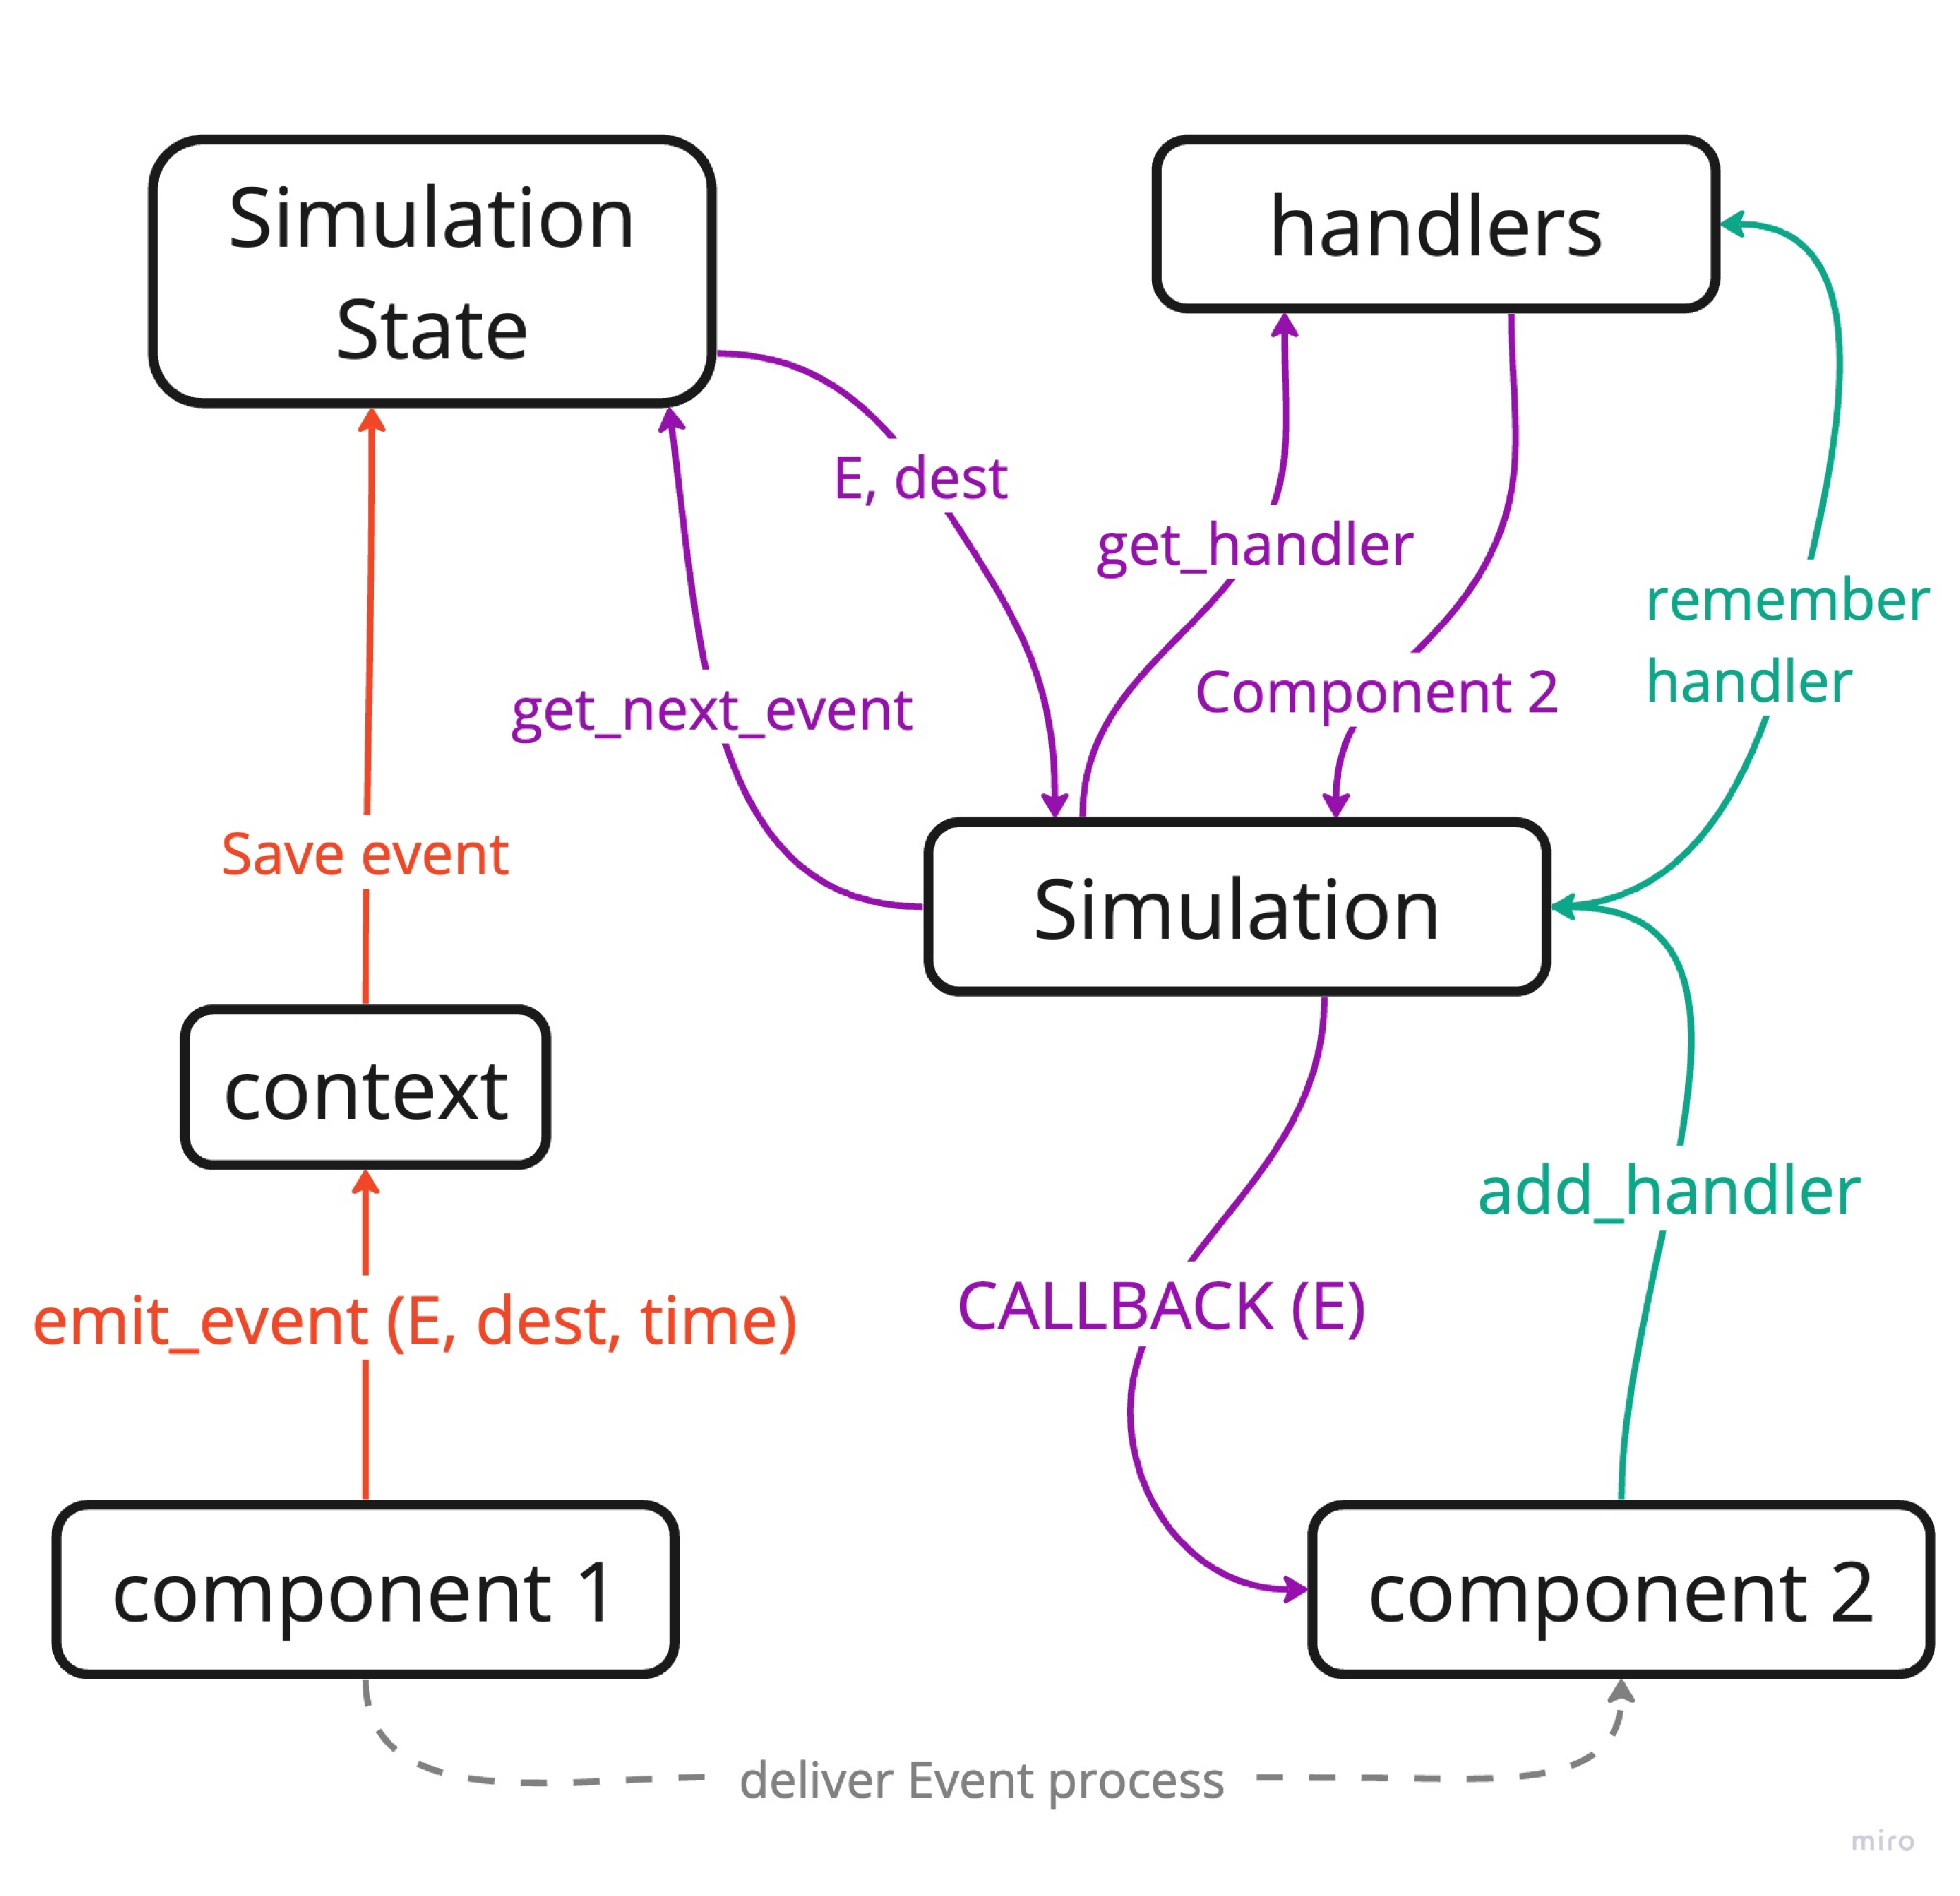
\includegraphics[width=0.7\linewidth]{images/dslab-core-callback.pdf}
    \caption{Реализация модели \texttt{callback} в \texttt{dslab-core}}
    \label{dslab_inner}
\end{figure}

На схеме \ref{dslab_inner} показан процесс доставки события от \texttt{Component~1} к \texttt{Component~2}. На картинке разными цветами обозначены процессы, происходящие в разное время. Сначала получатель должен зарегистрировать себя в симуляции (зеленый цвет на схеме \ref{dslab_inner}). Затем компонент-отправитель через свой контекст добавляет событие в симуляцию одним из методов \texttt{emit}, событие сохраняется в \texttt{SimulationState} и ожидает своего времени наступления (оранжевый цвет на схеме \ref{dslab_inner}). Когда на очередном шаге \hyperref[Simulation::step]{\texttt{Simulation::step}} приходит очередь это событие доставить, по нему определяется \texttt{handler} (компонент-получатель), и вызывается соответствующий \hyperref[fnon]{\texttt{callback}} с пользовательским кодом (фиолетовый цвет на схеме \ref{dslab_inner}). В процессе обработки этого события в симуляцию по точно такому же принципу добавляются новые, цикл замыкается.


\subsection{Асинхронная доставка событий}
Асинхронная схема доставки события состоит из большего числа шагов. Цепочки действий, происходящие в разное время снова отображены разными цветами. 
\nopagebreak
\begin{figure}[H]
    \centering
    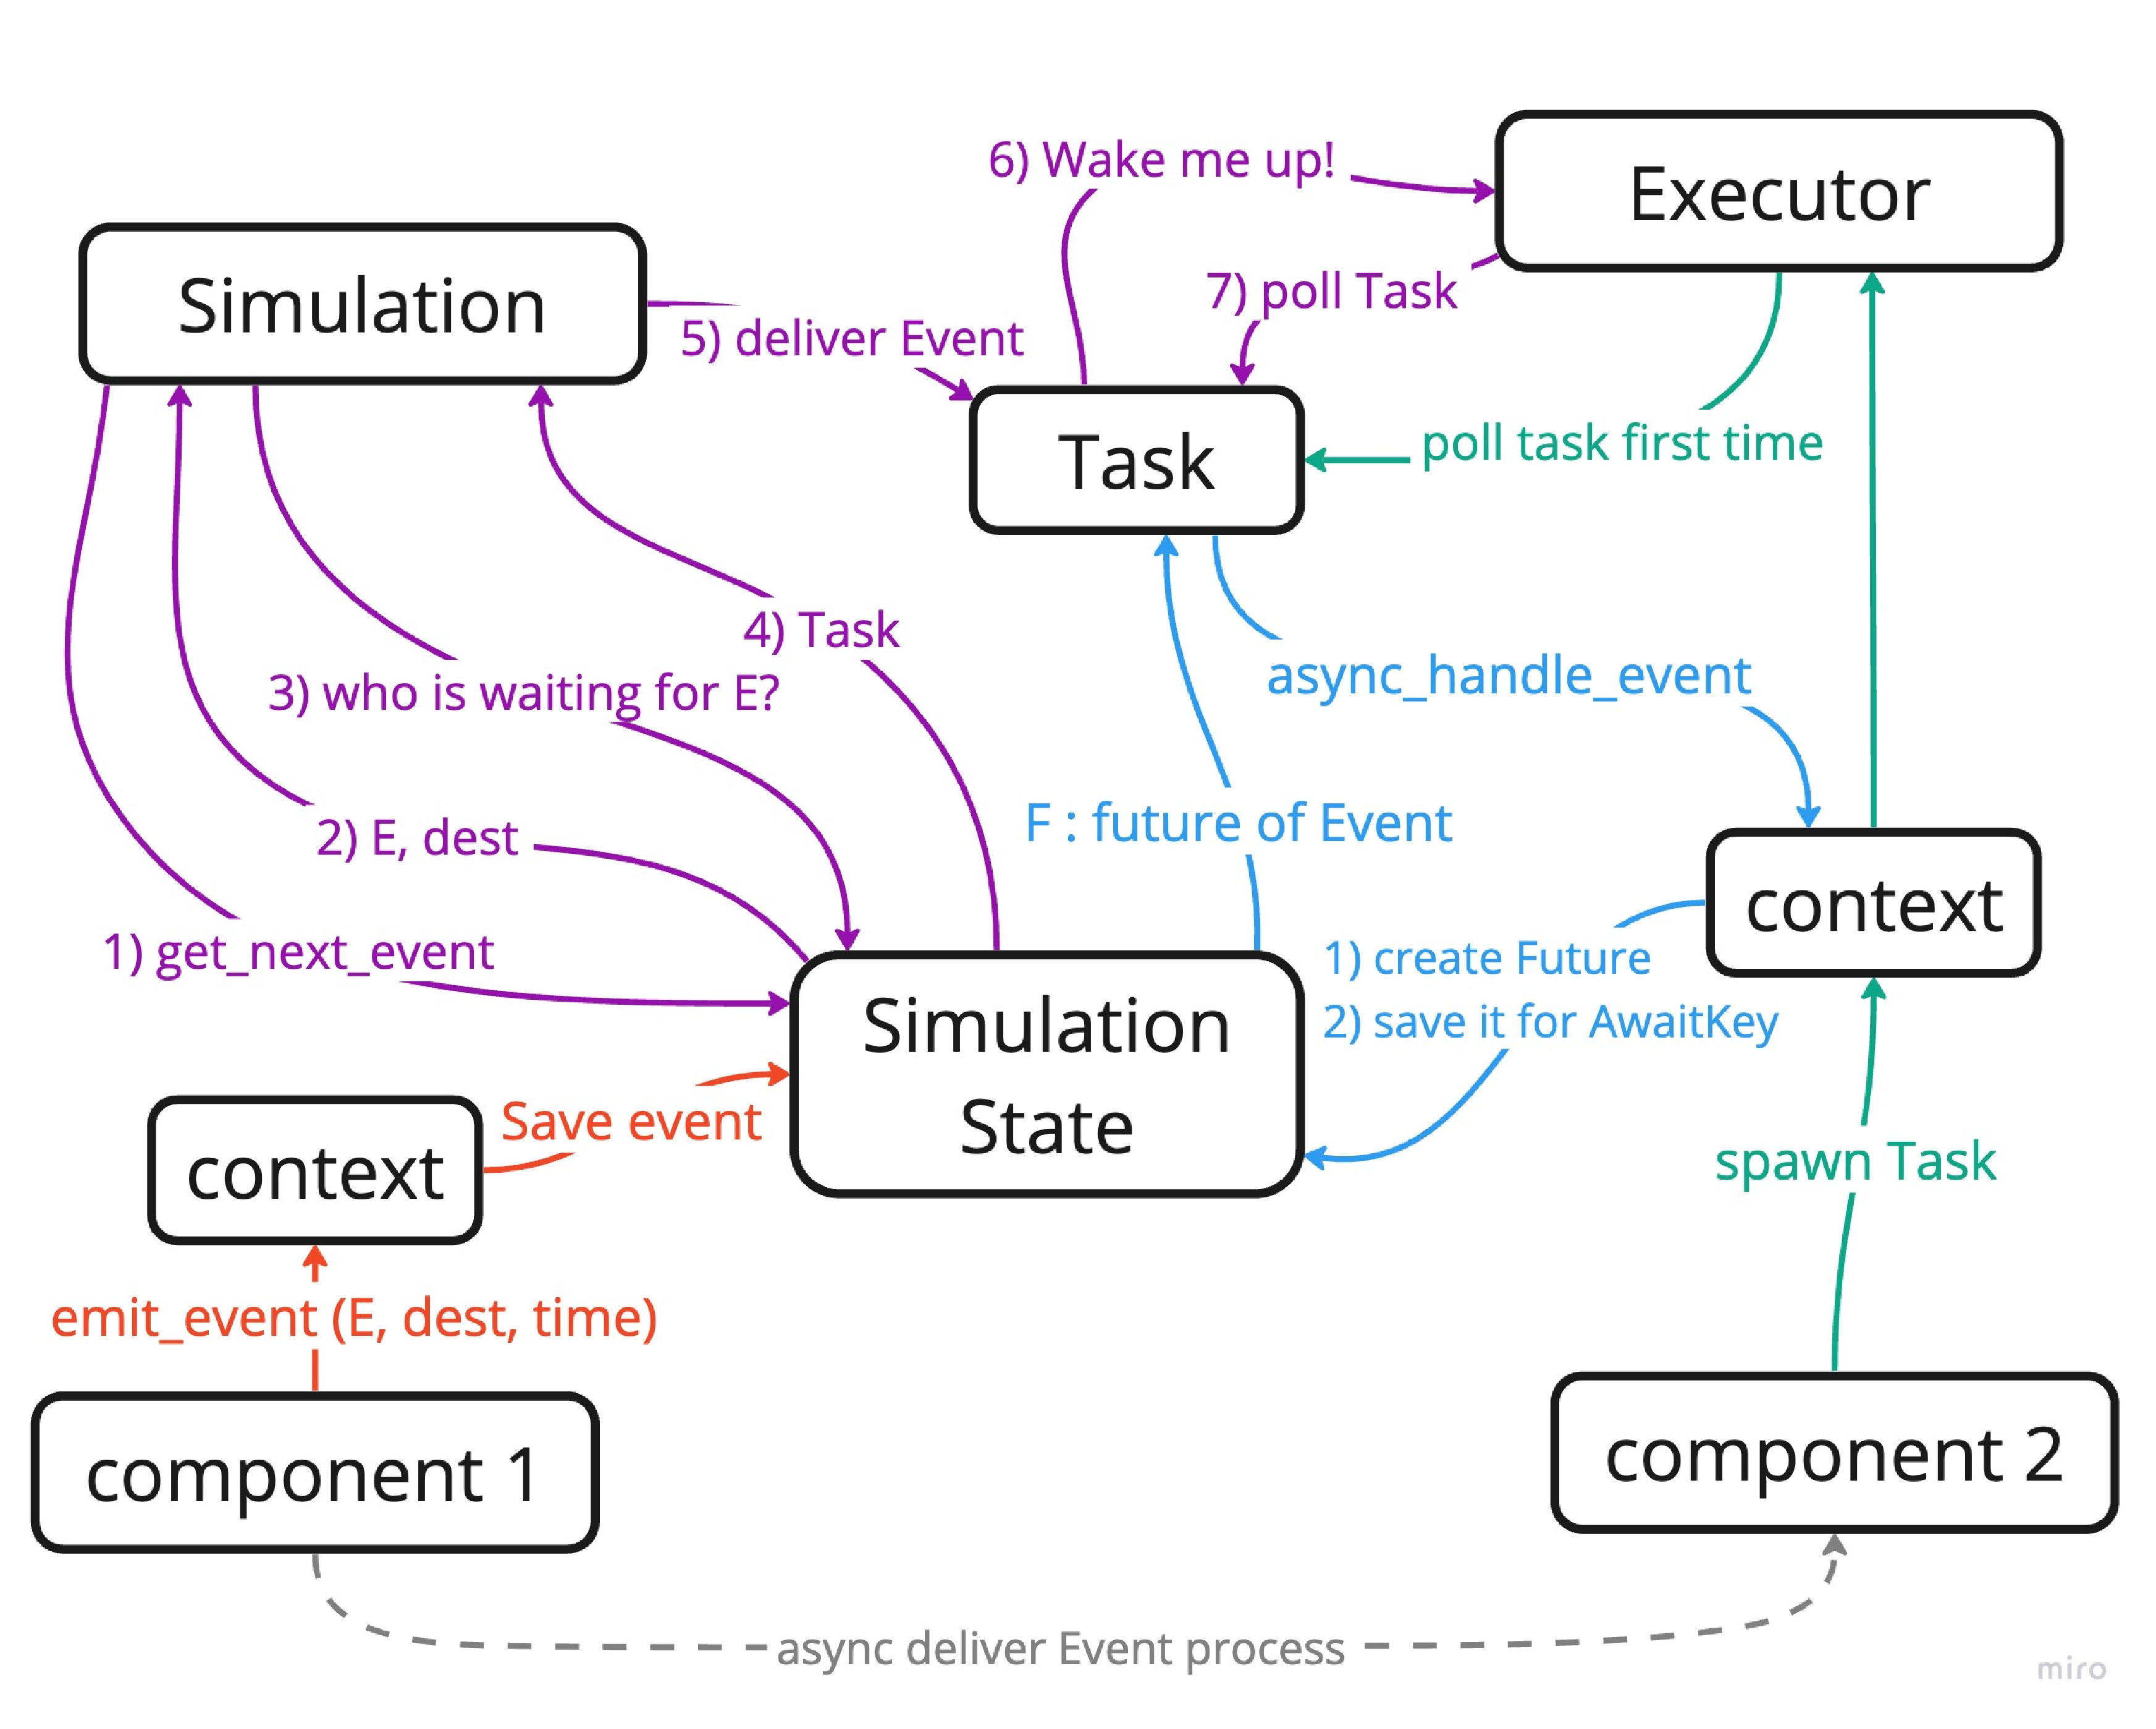
\includegraphics[width=\linewidth]{images/async-dslab-core-new.pdf}
    \caption{Реализация асинхронной модели доставки событий в \texttt{dslab-core}}
    \label{async_dslab_inner}
\end{figure}

\paragraph{Задача (Task)}
Любая асинхронная активность начинается с метода \hyperref[spawn]{\texttt{spawn}} (обозначено зеленым цветом на схеме \ref{async_dslab_inner}). Таким образом корневая асинхронная функция становится задачей, у которой будет возобновляться исполнение. Задача обладает способностью <<разбудить>> себя (хранит в себе ссылку на очередь задач и при вызове соответствующего метода добавляет себя в эту очередь, чтобы потом исполнитель задач ее исполнил). Именно задача является тем, кто ждет какое-либо событие для компонента. Для того чтобы асинхронно дождаться какого-то события нужно обратиться к \texttt{SimulationContext} за \texttt{Future} на это событие. При создании этого \texttt{Future} считается \hyperref[awaitkey]{AwaitKey}, полученная информация об ожидающей задаче сохраняется по ключу в \texttt{SimulationState}, ожидание начинается, задача прерывается (этот процесс обозначен синим цветом на схеме \ref{async_dslab_inner}). Процесс отправки события никак не отличается от классической модели \ref{dslab_inner}  -- событие попадает ровно в ту же очередь.

Стоит отметить, что метод \hyperref[spawn]{spawn} не порождает никаких параллельных активностей. Для детерминизма симуляции и воспроизводимости результатов все задачи выполняются строго последовательно.



\paragraph{Разделяемое состояние (SharedState)}
Чтобы передавать данные между \texttt{dslab-core} и пользовательским кодом асинхронно, у каждого \texttt{Future} есть разделяемое состояние -- ссылка на разделяемую структуру \texttt{AwaitEventSharedState} в динамической памяти. Эта ссылка сохраняется в \texttt{SimulationState} (на этапе создания \texttt{Future}, отмечен синим на схеме \ref{async_dslab_inner}) по вычисленному \hyperref[awaitkey]{ключу} ожидания, чтобы в эту <<корзинку>> можно было <<положить>> пришедшее событие (пункт 5 в процессе доставки сообщения, отмечен фиолетовым на схеме \ref{async_dslab_inner}). В конце процесса  доставки задача снова ставится на исполнение и событие <<достается>> из разделяемого состояния. 

\paragraph{Исполнитель задач (Executor)}
К полям \texttt{Simulation} добавляется еще одно поле -- \texttt{Executor}. Он предоставляет единственный метод: \texttt{fn process\_task()} -- выполнить первую в очереди задачу. Каждая задача может сама положить себя в очередь, когда ей будет доставлено событие (последние шаги \texttt{6} и \texttt{7} доставки события, отмечено фиолетовым цветом на схеме \ref{async_dslab_inner}) В случае, если асинхронная активность завершилась, ее объект нужно разрушить, чтобы не было утечек памяти. 

\paragraph{Процесс доставки события} Итого, часть отправки события полностью совпадает с классическим \texttt{callback} методом (обе части отмечены оранжевым цветом на схемах \ref{dslab_inner} и \ref{async_dslab_inner}). Главные различия происходят в методе \hyperref[Simulation::step]{\texttt{Simulation::step}} (также отмечен одинаковым фиолетовым цветом на обеих схемах). Опишем шаги этого метода а асинхронной модели доставки (со схемы \ref{async_dslab_inner}):
\begin{enumerate}
    \item[1-2.] Берется первое событие, которое должно наступить. 
    \item[3-4.] Происходит вычисление \hyperref[awaitkey]{\texttt{AwaitKey}} этого события.
    \begin{itemize} \item Если по такому ключу никто не ждет, переходим в классический режим \texttt{callback}-модели -- ищем нужный \texttt{handler} и вызываем \hyperref[fnon]{\texttt{callback}} как показано на схеме~\ref{dslab_inner}.
        \item Если нашлась ожидающая задача, то переходим к следующему пункту.
    \end{itemize}
    \item[5.] Доставляем событие в разделяемое состояние (которое мы нашли по ключу-ожидания).
    \item[6.] Добавляем задачу в очередь на исполнение \texttt{Executor}.
    \item[7.] Исполняем задачу. В процессе ее исполнения могут порождаться новые события, так цикл симуляции замыкается.  
\end{enumerate}

Это лишь краткое и наглядное описание реализации. Полный код реализации приведен форке репозитория \texttt{DSLab}\cite{async-dslab-core}. 
\section{Тестирование и замеры производительности} \label{async-testing}

\subsection{Ping-pong}

\texttt{Ping-pong} -- простейший пример, который можно реализовать в \texttt{DSLab}. Вместе с этим он является идеалом для того, чтобы протестировать производительность симуляции. В симуляции регистрируются определенное количество одинаковых компонентов, которые обмениваются между собой простыми сообщениями: отсылают \texttt{Ping}-сообщения своим <<соседям>> в случайном порядке, и на каждое \texttt{Ping}-сообщение отвечают сообщением \texttt{Pong}. Процесс повторяется много раз.

\subsubsection{Производительность}

Симуляция была запущена со следующими параметрами на рабочем ноутбуке:
\begin{table}[H]
    \centering
    \begin{tabular}{|c|c|c|c|c|c|c|}
        \hline
        Example & Hosts & Peers per host & Iterations & Elapsed time & Events/s & Iterations/s \\
        \hline
        async-ping-pong & 100000 & 100 & 100 & 16.45s & 1234103 & 6.08\\
        \hline
        ping-pong & 100000 & 100 & 100 & 8.20s & 2452670 & 12.20\\
        \hline
    \end{tabular}
    \caption{Сравнение производительности \texttt{async-ping-pong} и \texttt{ping-pong}}
    \label{cmp:ping-pong}
\end{table}

Видим двукратную деградацию в производительности. Естественно это связано с дополнительными расходами на асинхронность. Для каждого события необходимо посчитать его \hyperref[awaitkey]{AwaitKey}, доставить его в соответствующий \texttt{SharedState}, поставить задачу на исполнение в \texttt{Executor} и выполнить задачу.

Можем также пронаблюдать линейный рост потраченного времени на симуляцию с ростом количества итераций на графике \ref{async-perf}. Видно, что при общей тенденции на линейный рост времени есть небольшие выбросы, которые можно связать с работой на ноутбуке большого количества фоновых программ, влияющих на производительность системы:
\begin{figure}[H]
    \centering
    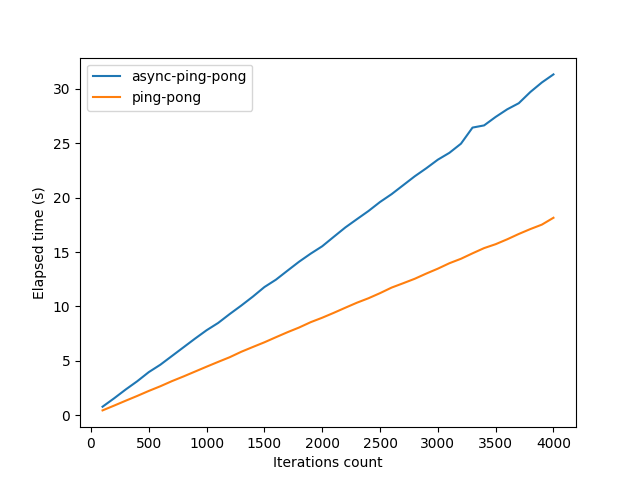
\includegraphics[width=0.9\linewidth]{images/async-ping-pong.png}
    \caption{Сравнение производительности примеров \texttt{ping-pong} и \texttt{async-ping-pong}}
    \label{async-perf}
\end{figure}

Однако, \texttt{ping-pong} -- это довольно вырожденный пример. Обычно значительное время работы симуляции занимает как раз работа пользовательского кода (в этом примере она полностью отсутствует). С точки зрения приближенности к реальным условиям показательнее будет следующий пример \ref{master-workers-subsection}. 

\subsubsection{Сравнение кода}

Пример довольно простой, но уже на нем можно увидеть радикальные различия в подходах. В синхронном примере первый \texttt{Ping} посылается на старте, есть функция реагирования на \texttt{Ping} сообщения, а при получении \texttt{Pong} посылается новый \texttt{Ping}. Код разделен на 3 отдельных участка (код намеренно упрощен для наглядности, полный пример можно смотреть в репозитории\cite{async-ping-pong-example}): 

\begin{figure}[H]
    \centering
    \begin{subfigure}[b]{0.40\linewidth}
        \footnotesize
        \centering
        \begin{rustcode}
pub struct Process {
  iterations: u32,
}

fn on_start(&mut self) {
  let peer = /*random peer*/;
  self.send(Ping {}, peer);
}
    \end{rustcode}
        \caption{Старт ping-pong}
        \label{start-ping-pong}
    \end{subfigure}
    \hfill
    \begin{subfigure}[b]{0.51\linewidth}
        \footnotesize
        \centering
        \begin{rustcode}
fn on_ping(&mut self, from: Id) {
  self.send(Pong {}, from);
}        
fn on_pong(&mut self, from: Id) {
  self.iterations -= 1;
  if self.iterations > 0 {
    let peer = /*choose peer*/
    self.send(Ping {}, peer);
  }
}
    \end{rustcode}
        \caption{Реакция на \texttt{Ping} и \texttt{Pong} сообщения}
        \label{ping-pong-on-pong}
    \end{subfigure}
\caption{\texttt{Ping-pong} example}
\label{ping-pong-code}
\end{figure}

Видно, что для того, чтобы сделать заданное количество итераций процесса \texttt{ping-pong}, нужно в полях структуры самого процесса хранить информацию о том, сколько их осталось. Эту роль выполняет переменная \texttt{iterations} (определяемая на участке кода \ref{start-ping-pong}). По трём отдельным участкам кода единого процесса работы не прослеживается. Его можно увидеть только внимательно вчитавшись в суть предоставленных \texttt{callback}-ов.

Теперь посмотрим, как абсолютно аналогичную задачу выполняет асинхронная реализация того же процесса (код также упрощен для наглядности, полный код можно смотреть в примере\cite{async-ping-pong-example}): 

\begin{figure}[H]
    \centering
    \begin{subfigure}[b]{0.45\linewidth}
        \footnotesize
        \centering
        \begin{rustcode}
fn on_start(&self) {
  self.ctx.spawn(
    self.process()
  );
}

fn on_ping(&mut self, from: Id) {
  self.send(Pong {}, from);
}    
    \end{rustcode}
        \caption{Старт процесса и callback на \texttt{Ping}}
        \label{start-async-ping-pong}
    \end{subfigure}
    \hfill
    \begin{subfigure}[b]{0.54\linewidth}
        \footnotesize
        \centering
        \begin{rustcode}
async fn process(&self) {
  for _i in 0..self.iterations {
    let peer = /*choose peer*/;
    self.send(Ping {}, peer);

    // stop execution until receive Pong
    self.ctx.async_handle_event::<Pong>(peer).await;
  }
}
    \end{rustcode}
    \caption{Асинхронная функция работы процесса}
    \label{async-ping-pong-action}
\end{subfigure}
\caption{\texttt{Async-ping-pong} example}
\label{async-ping-pong-code}
\end{figure}

Можно видеть, что код функции \texttt{process} (участок кода \ref{async-ping-pong-action}) очень четко выражает весь алгоритм работы. Особенно хорошо видна разница, сравнивая с функциями классической реализации \texttt{ping-pong} (участок кода \ref{ping-pong-on-pong}) -- там 2 отдельные функции, которые описывают только реакции, хотя на самом деле в симуляции происходит процесс, который идеально описывается циклом \texttt{for} (\ref{async-ping-pong-action}). 

Также этот пример демонстрирует обратную совместимость с моделью \texttt{callback}-ов. В случае, когда это уместно и выразительно, ее даже нужно использовать -- это видно на примере реакции на сообщения \texttt{Ping}, -- мы должны просто вернуть \texttt{Pong} отправителю (участок кода \ref{start-async-ping-pong}). 

\subsection{Master-workers}\label{master-workers-subsection}

Этот пример намного более сложный с точки зрения логики пользователя. Один компонент \texttt{Master} распределяет приходящие к нему задачи между большим количеством \texttt{Worker}-ов, каждый из которых выполняет длинный pipeline для каждой задачи. 

\subsubsection{Производительность}

Сравнивался существующий синхронный пример \texttt{master-workers} \cite{master-workers-example} с асинхронным аналогом \texttt{async-master-workers} \cite{async-master-workers-example}. Примеры различаются лишь подходом к обработке событий, логика и симуляция в примерах полностью совпадают. Оба примера были запущены с параметрами 100 хостов и 100000 задач. Получились такие результаты:

\begin{table}[H]
    \centering
    \begin{tabular}{|c|c|c|c|c|c|}
        \hline
        Example & Tasks & Hosts & Elapsed time & Scheduling time & Events per second \\
        \hline
        async-master-workers & 100000 & 100 & 5.97s & 4.31s & 285059 \\
        \hline
        master-workers & 100000 & 100 & 5.19s & 4.31s & 328392 \\
        \hline
    \end{tabular}
    \caption{Сравнение производительности \texttt{async-master-workers} и \texttt{master-workers}}
    \label{cmp:master-workers}
\end{table}

Тут как можно заметить результаты не такие разные (по сравнению с примером \hyperref[cmp:ping-pong]{\texttt{ping-pong}}), т.к. основное время тратится в пользовательской симуляции (на Scheduling time), а не на обмен событиями. Использование асинхронности никак не замедляет и не ускоряет пользовательский код. 


\subsubsection{Сравнение кода}

Приведем (в очень сжатом виде) сравнение семантики двух примеров. Полный код можно найти в репозитории (классическая реализация \texttt{master-workers}\cite{master-workers-example}, и асинхронная реализация \texttt{async-master-workers}\cite{async-master-workers-example}). На примере ниже показаны функции компонента \texttt{Worker} (исполняющего задачи).

\begin{figure}[H]
    \hspace{-0.55cm}
    \centering
    \begin{subfigure}[b]{0.537\linewidth}
        \footnotesize
        \centering
        \begin{rustcode}
pub struct Worker {
  tasks: HashMap<u64, TaskInfo>,
  computations: HashMap<u64, u64>,
  reads: HashMap<u64, u64>,
  writes: HashMap<u64, u64>,
  downloads: HashMap<usize, u64>,
  uploads: HashMap<usize, u64>,
}
fn on_task_request(request);
fn on_data_read_completed(request_id);
fn on_comp_started(comp_id);
fn on_comp_finished(comp_id);
fn on_data_write_completed(request_id);
fn on_data_transfer_completed(data);
    \end{rustcode}
        \caption{Выполнение задачи в \texttt{master-workers}}
        \label{master-workers}
    \end{subfigure}
    \hfill
    \begin{subfigure}[b]{0.48\linewidth}
        \footnotesize
        \centering
        \begin{rustcode}
fn on_task_request(req) {
  self.ctx.spawn(
    self.process_task_request(req));
}
async fn process_task_request(&self, req: TaskRequest) {
  let mut task = TaskInfo {req};

  self.download_data(&task).await;
  self.read_data(&task).await;
  self.run_task(&task).await;
  self.write_data(&task).await;
  self.upload_result(&task).await;
}
    \end{rustcode}
    \caption{Пайплайн задачи в \texttt{async-master-workers}}
    \label{async-master-workers}
\end{subfigure}
\caption{Сравнение \texttt{master-workers} и \texttt{async-master-workers}}
\label{master-workers-comparison}
\end{figure}

На этом примере видно схожую разницу, только в большем масштабе. В классическом случае с \texttt{callback}-ами мы вынуждены хранить промежуточную информацию о процессе выполнения всех задач в полях структуры \texttt{Worker} (код \ref{master-workers}). Это приводит к нагромождению кода операциями по чтению и записи в эти общие структуры. Более того, по набору декларируемых \texttt{callback}-ов непонятно, как они вообще связаны, в каком порядке должны идти. Об это можно догадываться по названиям, но чтобы узнать точно, нужно подробно вчитаться, что делает \texttt{Worker} в каждом из \texttt{callback}-ов. Отдельное неудобство конкретно в этом примере доставляет то, что \texttt{callback} \texttt{\underline{on\_data\_transfer\_completed}} (код \ref{master-workers}) вызывается компонентом сети дважды при выполнении одной задачи: после загрузки изначальных данных и после выгрузки результатов, что порождает необходимость ставить внутри условия.  

Как с этим справляется асинхронный код можно видеть на примере \ref{async-master-workers}. На запрос задачи все еще реагирует \texttt{callback} (что является здесь вполне уместным), но процесс выполнения устроен совершенно по-другому. Сразу видна последовательность действий, прогресс задачи сохранен в <<локальной>> переменной и не перегружает структуру \texttt{Worker}. Для того чтобы узнать подробности каждого этапа нужно пройти в соответствующие функции (внутри которых тоже есть асинхронные ожидания). 

При более внимательном рассмотрении можно увидеть, что код \ref{master-workers} в первом приближении является развернутой \texttt{state-machine} кода \ref{async-master-workers} (по аналогии с примером \ref{sync-async-example}). Как раз это <<разворачивание>> делает за нас компилятор \texttt{Rust}, позволяя нам писать <<синхронный>> выразительный код.

Из-за полной обратной совместимости с моделью \texttt{callback}-ов, код компонента \texttt{Master} остался без изменений, как и все используемые в этом примере зависимости (\texttt{Network}, \texttt{Disk}, \texttt{ComputeMulticore}).

\subsection{Event-details}
Пример является немного упрощенной версией \texttt{master-workers} (раздел \ref{master-workers-subsection}): один хост разбирает поступающие задачи и ставит их параллельно на свой процессор (подключенный модуль \texttt{ComputeMulticore}). Смысл примера в демонстрации нескольких новых функций: реализованного стандартного примитива синхронизации \hyperref[blockingqueue]{\texttt{UnboundedBlockingQueue<T>}} и альтернативного ожидания с помощью макроса \texttt{select!} из пакета \texttt{futures}. Сделать краткую содержательную выжимку кода этого примера довольно трудно, поэтому с ним можно подробно ознакомиться в репозитории\cite{async-event-details-example}.

Основная идея состоит в том, что при старте вычислительной активности модуль \texttt{ComputeMulticore} присылает либо событие \texttt{CompStarted} (если удалось выделить ресурсы и начать исполнять задачу) либо событие \texttt{CompFailed} (если процессор сейчас слишком нагружен для такой задачи). Именно такое альтернативное ожидание используется в примере. Если получили \texttt{CompFailed}, то нужно дождаться завершения любого другого вычислительного процесса и попробовать снова. 

\texttt{UnboundedBlockingQueue<T>} используется для удобного сохранения задач в очереди. \texttt{Сallback} \texttt{\underline{fn on\_task\_request}} складывает сообщение в очередь, а процесс \texttt{async fn work\_loop} достает, когда это нужно, или блокируется в ожидании следующей задачи.

\section{Заключение}

Разработанное асинхронное расширение для ядра идеально дополняет старый подход, а не является альтернативой. Строго говоря, классическую модель \texttt{callback}-ов можно целиком выразить новыми средствами асинхронности, однако это не принесет никаких преимуществ, только симуляция будет работать медленнее (как показал пример \hyperref[cmp:ping-pong]{\texttt{ping-pong}}). По примерам разобранным в главе \ref{async-testing} можно проследить четкую закономерность: для \texttt{Stateless}-процессов\footnote{
    \texttt{Stateless}-процесс не нуждается в хранении никакого состояния и может быть выполнен сразу целиком, не имеет побочных эффектов, которые нужно было бы сохранять. Классический пример -- ответить сообщением \texttt{Pong} на сообщение \texttt{Ping} (код \ref{start-async-ping-pong}). }
лучше и интуитивнее работает подход \texttt{callback}-ов, а для \texttt{Stateful}-процессов\footnote{
    \texttt{Stateful}-процессы выполняются в несколько этапов и требуют сохранения промежуточного состояния между этими этапами. Из разобранных примеров самым наглядным является пайплайн выполнения задачи в \texttt{async-master-workers} (код \ref{async-master-workers})} 
асинхронность оказывается намного выразительнее и удобнее. В рамках одной симуляции часто приходится работать с большим разнообразием процессов, комбинируя использование асинхронного и классического подхода. Именно возможность бесшовной интеграции со старыми компонентами, используя при этом новые методы по необходимости, является главным достижением этой работы.



\subsection{Характеристика результатов работы}

В результате было разработано рабочее расширение ядра \texttt{dslab-core}\cite{async-dslab-core} и написаны примеры его использования\cite{async-ping-pong-example}\cite{async-event-details-example}\cite{async-master-workers-example}. Основной функционал покрыт тестами. В тексте этой работы приведено наглядное сравнение подходов (глава \ref{async-testing}).

Таким образом, главная \hyperref[main-purpose]{цель} проекта достигнута,  выполнены основные \hyperref[requirements]{требования}. 

\subsection{Планы на будущее} \label{future-plans}
Будущее развитие проекта можно разделить на 4 направления: 
\begin{itemize}
    \item \underline{Повышение удобства синтаксиса.} Например, сейчас для использования детализированного ожидания необходимо для каждого типа событий регистрировать функцию по получению этих самых деталей (часть \ref{add-details-getters}), что является, на первый взгляд, избыточным. Почти наверняка эту функцию можно красиво и эффективно реализовать с помощью макросов языка \texttt{Rust}. Это один из примеров возможного улучшения в этой области. 
    \item \underline{Увеличение производительности симуляции.} Для этого нужно еще более глубоко погрузиться во внутренне устройство рантайма языка \texttt{Rust}, чтобы найти потенциально неэффективные места. Возможно также применить профилирование программы и другие методы диагностики производительности программы. Это самая сложная область дальнейшей деятельности. 
    \item \underline{Расширение асинхронной функциональности.} Чтобы сделать расширенное ядро еще более выразительным, в него можно добавить, например, функцию \texttt{yield} -- <<уйти в конец очереди планировщика>>. Это техническая функция позволит сначала обработать все события текущего времени в симуляции, а затем уже продолжить исполнение текущей задачи. Это может быть полезно для реализации более сложных асинхронных алгоритмов и примитивов синхронизации, которые завязаны на передаче управления друг другу без продвижения симуляции по времени. 
    
    Другим возможным расширением асинхронной функциональности будет являться \\ \texttt{cancellation} -- отмена работающих процессов. Это может сильно упростить написание распределенных алгоритмов, где отмены задач являются частым явлением. \texttt{Cancellation}~-- достаточно сложный вопрос с точки зрения правильного дизайна, который нужно будет тщательно продумать перед реализацией.
    
    Также расширение асинхронной функциональности является предметом исследования. Скорее всего при накоплении опыта использования появятся новые запросы или откроются проблемы, которые нужно будет решать.
    \item \underline{Расширение <<стандартных>> асинхронных инструментов.} После появления метода \texttt{yield} станет возможным реализовать полноценный канал передачи данных из языка \texttt{Go}. Такой канал мог бы стать универсальным примитивом синхронизации и  идеально дополнял бы асинхронный фреймворк. Однако, его реализация -- непростая задача из-за большого количества возможных случаев, которые необходимо будет рассмотреть.  
    
    Еще возможна реализация примитива \texttt{condition\_variable}, но его применение видится существенно более ограниченным и специфичным чем \texttt{Go}-like канала.

    В этом пункте также не исключена исследовательская составляющая и появление новых задач с накоплением опыта использования фреймворка.
\end{itemize}





\newpage
\addcontentsline{toc}{section}{Список источников}

\Urlmuskip=0mu plus 1mu\relax

\printbibliography

% \addcontentsline{toc}{section}{Список иллюстраций}
% \listoffigures


\end{document}
% Начиная с этого момента весь текст LaTeX игнорирует, можете вставлять любую абракадабру.
